%This is a template file for use of iopjournal.cls

\documentclass{iopjournal}

% Options
%  [anonymous]  Provides output without author names, affiliations or acknowledgments to facilitate double-anonymous peer-review

\usepackage{cite}
\usepackage{amsmath,amssymb,amsfonts}
\usepackage{algorithmic}
\usepackage{graphicx}
\usepackage{textcomp}
\usepackage{xcolor}
\usepackage{booktabs}
\usepackage{hyperref}
\usepackage{float}

\begin{document}

\articletype{Paper}

\title{Sistem Terintegrasi Deteksi dan Pengukuran Lubang Jalan Menggunakan YOLOv8 dan DepthAnything V2 dengan Filter Temporal}

\author{Pangeran Juhrifar Jafar}
\affil{Jurusan Sistem Informasi, Universitas Hasanuddin, Makassar, Indonesia}
\email{pangeranjuhrifar@gmail.com}

\keywords{Deteksi Lubang Jalan, Estimasi Kedalaman Monokuler, YOLOv8m-seg, DepthAnything V2, Kalman Filter, Smart City, Inspeksi Jalan Otomatis}

\begin{abstract}
Pemeliharaan jalan yang proaktif sangat penting untuk keselamatan dan efisiensi ekonomi, namun metode inspeksi manual masih bersifat reaktif, subjektif, dan berisiko. Makalah ini menghadirkan sistem terintegrasi untuk deteksi dan pengukuran lubang jalan secara \textit{real-time} menggunakan perangkat \textit{edge}. Sistem memadukan \textbf{YOLOv8m-seg} untuk deteksi dan segmentasi instan, \textbf{DepthAnything V2} untuk estimasi kedalaman monokuler, serta penyaringan temporal untuk stabilitas pengukuran.

\textit{Pipeline} mencakup: (1) deteksi lubang dengan segmentasi instansi; (2) estimasi kedalaman dan pemulihan skala berbasis tinggi kamera untuk memperoleh ukuran metrik absolut; (3) pengukuran diameter dan kedalaman menggunakan statistik robust dan penyesuaian mask; (4) pelacakan BoT-SORT dan penyaringan \textbf{Confidence and Distance Kalman Filter (CDKF)} untuk menstabilkan estimasi; (5) pelaporan otomatis melalui REST API.

Evaluasi menunjukkan sistem mampu berjalan pada $\sim$30 FPS dengan kesalahan pengukuran di bawah 15\%. Hasil ini menegaskan kelayakan sistem sebagai solusi inspeksi jalan cerdas di lingkungan dengan sumber daya terbatas, sekaligus menyediakan data bernilai tinggi untuk pemeliharaan infrastruktur secara proaktif.
\end{abstract}


\section{Pendahuluan}
\label{sec:introduction}

Infrastruktur jalan memainkan peran penting dalam mobilitas, pertumbuhan ekonomi, dan akses layanan publik. Namun, menjaga kualitas jalan merupakan tantangan besar, terutama di negara dengan kondisi geografis kompleks seperti Indonesia. Menurut Kementerian PUPR, sekitar 30\% dari 496.000 km jaringan jalan nasional mengalami kerusakan dari ringan hingga berat \cite{kemenpupr}. Di antara berbagai jenis kerusakan, lubang jalan adalah salah satu yang paling umum dan berbahaya karena dapat menyebabkan kecelakaan, kerusakan kendaraan, dan kerugian ekonomi.

Deteksi kerusakan jalan secara tradisional mengandalkan inspeksi manual dan laporan masyarakat, yang bersifat reaktif, padat karya, dan rentan kesalahan subjektif. Kebutuhan akan sistem deteksi otomatis yang akurat dan berkelanjutan semakin mendesak seiring perkembangan teknologi \textit{smart city}. Meskipun model deteksi berbasis CNN—seperti YOLO—telah menunjukkan performa tinggi dalam deteksi lubang secara \textit{real-time} \cite{gorro2024}, deteksi saja tidak cukup untuk perencanaan pemeliharaan. Pengukuran dimensi lubang (diameter dan kedalaman) sangat penting untuk menentukan prioritas perbaikan dan estimasi volume material.

Pendekatan sensor 3D seperti LiDAR atau stereo mampu menghasilkan kedalaman yang akurat tetapi memiliki kendala biaya dan komputasi. Estimasi kedalaman monokuler menjadi alternatif yang efisien, namun menghadapi tantangan utama yaitu \textit{scale ambiguity}. Penelitian terbaru seperti Wang et al. \cite{wang2025} mulai mengatasi isu ini melalui pemrosesan temporal, tetapi integrasi penuh ke dalam sistem inspeksi \textit{real-time} masih terbuka untuk ditingkatkan.

Makalah ini mengusulkan sebuah sistem terintegrasi yang menggabungkan model deteksi modern dengan estimasi kedalaman dan penyaringan temporal untuk menghasilkan pengukuran lubang jalan yang stabil dan akurat. Kontribusi utama penelitian ini adalah:
\begin{enumerate}
    \item Sistem deteksi \textit{real-time} berbasis \textbf{YOLOv8m-seg} dengan segmentasi instansi untuk akurasi area yang lebih tinggi.
    \item Modul estimasi kedalaman monokuler menggunakan \textbf{DepthAnything V2} dengan pemulihan skala berbasis tinggi kamera.
    \item Teknik pengukuran berbasis statistik robust dan \textit{ellipse fitting} pada mask segmentasi untuk memperoleh diameter dan kedalaman metrik.
    \item Integrasi \textbf{BoT-SORT} dan \textbf{Confidence and Distance Kalman Filter (CDKF)} untuk memastikan konsistensi temporal pengukuran.
    \item Pipeline pelaporan otomatis ke dasbor manajemen infrastruktur melalui REST API dengan metadata komprehensif.
\end{enumerate}

Sisa makalah disusun sebagai berikut: Bagian II menjelaskan metodologi, Bagian III menyajikan hasil eksperimen dan analisis, dan Bagian IV memberikan kesimpulan dan arah penelitian selanjutnya.

\section{Metode}

Kerangka kerja yang diusulkan dirancang sebagai sistem terintegrasi untuk mendeteksi lubang jalan, menghitung karakteristik fisiknya, dan menyampaikan hasil pengukuran secara otomatis. Gambar~1 menunjukkan alur lengkap pipeline. Pertama, aliran video yang diperoleh dari kamera diproses oleh modul deteksi berbasis YOLOv8m-seg untuk mengidentifikasi lokasi lubang jalan dan menghasilkan representasi mask segmentasi yang presisi. Hasil deteksi ini kemudian diolah oleh algoritma BoT-SORT, yang menetapkan identitas unik bagi setiap lubang dan mempertahankan konsistensi pelacakan antar-frame.

Secara paralel, frame yang sama dianalisis oleh model estimasi kedalaman monokuler DepthAnything V2 untuk menghasilkan peta kedalaman secara densitas penuh. Informasi kedalaman dan segmentasi selanjutnya digabungkan dalam tahap pengukuran geometris, di mana diameter serta kedalaman lubang dihitung melalui pendekatan statistik yang dirancang untuk meminimalkan pengaruh \textit{noise}. Hasil pengukuran yang telah distabilkan diproses lebih lanjut dan dikemas dalam format terstruktur sebelum dikirimkan ke server melalui API untuk keperluan pemantauan atau pengambilan keputusan.

Gambar~1: Diagram alur keseluruhan kerangka kerja yang diusulkan.

Akhirnya, untuk meningkatkan ketahanan sistem terhadap fluktuasi temporal, ukuran lubang yang diperkirakan pada frame-frame berturut-turut diproses menggunakan Confidence-and-Distance Kalman Filter (CDKF). Filter ini mengintegrasikan tingkat kepercayaan deteksi serta jarak objek terhadap kamera sebagai komponen ketidakpastian dalam pemodelan, sehingga menghasilkan estimasi dimensi lubang jalan yang lebih stabil, konsisten, dan dapat diandalkan dari waktu ke waktu.


\subsection{Pengumpulan dan Anotasi Dataset}

Gambar 2
Penelitian ini menggunakan kombinasi dataset publik dan data lokal untuk memperoleh keragaman visual yang dibutuhkan dalam proses pelatihan model deteksi lubang jalan. Dataset publik utama diperoleh dari platform Roboflow Universe, yang menyediakan kumpulan dataset \textit{instance segmentation} lubang jalan dari berbagai kontributor global. Keragaman sumber data ini menghasilkan variasi signifikan pada tekstur jalan, kondisi pencahayaan, sudut pengambilan gambar, serta tingkat keparahan kerusakan, sehingga mendukung peningkatan kemampuan generalisasi model.

Untuk memastikan sistem tetap adaptif terhadap karakteristik lingkungan lokal, dataset publik tersebut dilengkapi dengan data tambahan yang direkam menggunakan kamera \textit{dashcam} dan kamera telepon seluler pada kondisi nyata di lapangan. Pengambilan data dilakukan pada berbagai jenis permukaan jalan, variasi cuaca, serta intensitas lalu lintas yang berbeda, sehingga mencerminkan kondisi jalan Indonesia yang heterogen.

Seluruh anotasi menggunakan format YOLO dengan kelas tunggal “pothole”. Karena penelitian ini menargetkan estimasi metrik yang presisi, anotasi dilakukan menggunakan \textit{instance segmentation mask} alih-alih \textit{bounding box} berbentuk persegi. Masker memungkinkan representasi kontur lubang jalan yang lebih akurat, yang sangat penting untuk proses pengukuran diameter berbasis proyeksi kamera dan estimasi kedalaman berbasis peta kedalaman.

Dataset gabungan kemudian dibagi menjadi tiga subset: pelatihan (80\% atau 2697), validasi (9\% atau 300), dan pengujian (11\% atau 355), dengan mempertahankan keberagaman domain pada setiap subset. Untuk data lokal, metadata tambahan seperti \textit{timestamp}, koordinat GPS, dan parameter kalibrasi kamera dicatat selama proses akuisisi. Informasi ini digunakan pada tahap rekonstruksi kedalaman serta evaluasi spasial yang membutuhkan konsistensi geometris.

\subsection{Pra-pemrosesan dan Kalibrasi Kamera}
Sistem ini menggunakan kamera telepon seluler sebagai sumber utama akuisisi video. Kamera ponsel umumnya memiliki distorsi lensa yang lebih besar dibandingkan kamera industri, sehingga tahap pra-pemrosesan menjadi sangat penting untuk menjaga akurasi pengukuran geometris. Setiap \textit{frame} terlebih dahulu melalui proses koreksi distorsi lensa (\textit{lens undistortion}) guna menghilangkan efek distorsi radial dan tangensial yang dapat mengubah bentuk lubang jalan pada citra.

Kalibrasi kamera dilakukan menggunakan model kamera \textit{pinhole}. Parameter intrinsik yang meliputi matriks kamera $K$ serta koefisien distorsi $D$ diperoleh melalui proses kalibrasi menggunakan pola papan catur (\textit{checkerboard}) yang direkam langsung oleh kamera ponsel. Proses ini menghasilkan estimasi koefisien distorsi radial ($k_1, k_2, k_3$) dan distorsi tangensial ($p_1, p_2$), yang kemudian digunakan untuk memetakan ulang piksel sehingga menghasilkan citra yang telah terkoreksi secara geometris.

Setelah koreksi distorsi, citra kemudian dinormalisasi ukurannya sesuai kebutuhan masing-masing model. Frame untuk deteksi lubang diubah menjadi $640 \times 640$ piksel untuk kompatibilitas dengan arsitektur YOLOv8m-seg, sedangkan frame untuk estimasi kedalaman dipertahankan pada resolusi asli kamera atau disesuaikan menjadi $518 \times 518$ piksel mengikuti konfigurasi DepthAnything V2. Pemisahan jalur resolusi ini memastikan kedua model menerima kualitas informasi visual yang optimal tanpa mengorbankan detail tekstur yang diperlukan dalam rekonstruksi kedalaman.

\subsection{Arsitektur Model Deteksi dan Segmentasi}
Tahap deteksi lubang jalan dilakukan menggunakan model \textbf{YOLOv8m-seg}, yaitu varian medium dari keluarga YOLOv8 yang dirancang khusus untuk kebutuhan segmentasi instans dengan keseimbangan akurasi yang lebih baik. Model ini dipilih karena memiliki keseimbangan optimal antara akurasi dan kecepatan, sehingga memungkinkan proses inferensi secara \textit{real-time} pada perangkat kelas konsumen seperti ponsel atau \textit{edge device} berperforma terbatas.

Pelatihan model dilakukan melalui pendekatan \textit{transfer learning} dengan menggunakan bobot pra-latih pada dataset COCO sebagai titik awal, kemudian di-\textit{fine-tune} menggunakan dataset lubang jalan yang terdiri dari kombinasi data publik dan data lokal. Pendekatan ini memungkinkan model mengadaptasi pola tekstur jalan dan kontur lubang dengan lebih cepat tanpa memerlukan pelatihan dari awal.

Berbeda dengan model deteksi berbasis kotak batas konvensional, YOLOv8m-seg tidak hanya memberikan prediksi \textit{bounding box} $(x, y, w, h)$, tetapi juga menghasilkan \textbf{mask segmentasi instans} yang mengikuti bentuk lubang jalan secara presisi. Masker ini sangat penting dalam pipeline pengukuran, karena:

\begin{enumerate}
    \item menghilangkan area latar belakang yang dapat mengganggu estimasi kedalaman,
    \item memastikan hanya piksel yang benar-benar berada di dalam lubang yang digunakan dalam perhitungan statistik kedalaman,
    \item memungkinkan pengukuran diameter melalui \textit{ellipse fitting} yang lebih akurat dibandingkan pendekatan berbasis bounding box.
\end{enumerate}

Dengan demikian, YOLOv8m-seg berfungsi sebagai fondasi utama yang menyediakan area \textit{Region of Interest} (ROI) berkualitas tinggi untuk tahap estimasi kedalaman dan pengukuran dimensi fisik pada langkah-langkah berikutnya.

\subsection{Estimasi Kedalaman Monokuler dan Pemulihan Skala}
Untuk mendapatkan informasi 3D dari citra 2D, kami menggunakan \textbf{DepthAnything V2} \cite{depthanything2024}, sebuah model berbasis \textit{Dense Prediction Transformer} (DPT) yang mampu menghasilkan peta kedalaman (\textit{depth map}) yang detail dan tahan terhadap variasi tekstur. Namun, model ini secara inheren menghasilkan kedalaman relatif (\textit{up-to-scale}) yang tidak memiliki satuan metrik \cite{florea2025}.

Untuk mengatasi masalah ambiguitas skala ini, kami mengajukan metode \textit{Height-Based Scale Recovery}. Dengan asumsi area jalan di depan kendaraan adalah bidang datar (\textit{flat ground assumption}), kami memanfaatkan tinggi pemasangan kamera ($H_{cam}$) yang diketahui sebagai referensi geometris. Faktor skala $S$ dihitung secara dinamis dengan membandingkan jarak absolut teoretis ke permukaan jalan dengan prediksi kedalaman relatif model pada \textit{Region of Interest} (ROI) jalan yang aman.

\begin{equation}
S = \frac{d_{abs\_road}}{d_{rel\_road}} = \frac{H_{cam} / \sin(\theta)}{Median(D_{rel}[ROI_{road}])}
\end{equation}

dimana $\theta$ adalah sudut \textit{pitch} kamera, dan $D_{rel}[ROI_{road}]$ adalah nilai kedalaman relatif pada area jalan di bagian bawah \textit{frame}. Peta kedalaman absolut kemudian diperoleh dengan $D_{abs} = S \times D_{rel}$.

\subsection{Pengukuran Dimensi Lubang dengan Statistik Robust}
Peta kedalaman yang dihasilkan oleh model monokuler seringkali mengandung \textit{noise} dan anomali, terutama pada area transisi atau objek dengan tekstur kompleks. Untuk memastikan pengukuran dimensi lubang yang akurat dan andal, kami mengadopsi pendekatan statistik robust. Metode ini dirancang untuk meminimalkan dampak \textit{outlier} dan variasi data yang tidak diinginkan, sehingga menghasilkan estimasi yang lebih stabil dan representatif.

Secara spesifik, pengukuran diameter lubang didasarkan pada analisis \textit{segmentation mask} yang dihasilkan oleh YOLOv8m-seg. Dari mask ini, dimensi spasial seperti panjang dan lebar maksimum dapat diekstraksi, atau bahkan fitting elips untuk mendapatkan sumbu mayor dan minor. Sementara itu, estimasi kedalaman lubang memanfaatkan nilai median dari distribusi kedalaman piksel dalam area yang relevan, yang secara efektif mereduksi pengaruh \textit{noise} dan memastikan bahwa kedalaman yang dilaporkan mencerminkan kondisi sebenarnya dari lubang. Penerapan teknik pemfilteran temporal dan statistik robust semacam ini telah terbukti efektif dalam meningkatkan ketahanan pengukuran kedalaman monokuler terhadap inkonsistensi frame-to-frame \cite{wang2025}.

Secara matematis, estimasi diameter ($D$) dan kedalaman efektif ($H$) diformulasikan sebagai berikut:

\begin{equation}
D = \frac{L_{major} \times \bar{Z}_{local}}{f_x}, \quad H = \tilde{Z}_{surface} - P_{10}(\{z \in \Omega_{roi} \mid Q_1 - 1.5 \text{IQR} \le z \le Q_3 + 1.5 \text{IQR}\})
\end{equation}

dimana $L_{major}$ adalah sumbu mayor dari elips yang di-fitting pada mask lubang, $\bar{Z}_{local}$ adalah kedalaman rata-rata lokal, $f_x$ adalah panjang fokus kamera. Untuk kedalaman, $\tilde{Z}_{surface}$ adalah median kedalaman permukaan jalan, dan dasar lubang ditentukan oleh persentil ke-10 ($P_{10}$) dari set kedalaman ROI ($\Omega_{roi}$) yang telah dibersihkan dari \textit{outlier} menggunakan metode \textit{Interquartile Range} (IQR).


\subsubsection{Estimasi Kedalaman Lubang}
\mbox{}\\
Kedalaman lubang ($d_{pothole}$) secara formal didefinisikan sebagai selisih jarak ortogonal antara bidang permukaan jalan rata-rata ($Z_{surface}$) dan taksiran dasar lubang ($Z_{base}$). Mengingat sifat \textit{noisy} dari estimasi kedalaman monokuler, pendekatan statistik digunakan untuk kedua variabel:

\begin{equation}
d_{pothole} = Z_{surface} - Z_{base}
\end{equation}

\begin{itemize}
    \item \textbf{Permukaan Jalan ($Z_{surface}$):} Dihitung menggunakan estimator robust median pada himpunan piksel dalam area \textit{border} ($\Omega_{border}$) selebar 10 piksel yang mengelilingi mask deteksi. Teknik ini, yang disarankan oleh Zhang et al. \cite{zhang2020} untuk rekonstruksi permukaan jalan, efektif mengeliminasi anomali topologi lokal.
    \begin{equation}
    Z_{surface} = \text{Median}(\{D(p) \mid p \in \Omega_{border}\})
    \end{equation}
    
    \item \textbf{Dasar Lubang ($Z_{base}$):} Ditentukan dari \textit{Region of Interest} ($\Omega_{roi}$) lubang. Alih-alih menggunakan nilai minimum yang rentan terhadap \textit{noise} sensor, kami menerapkan filter statistik dua tahap. Distribusi kedalaman disaring menggunakan \textit{Interquartile Range} (IQR) untuk menghapus \textit{outlier}, diikuti dengan pengambilan persentil ke-10 ($P_{10}$). Metode ini memberikan estimasi dasar yang konservatif namun akurat, seperti yang divalidasi dalam studi inspeksi infrastruktur oleh Bentzer \cite{bentzer2025}.
    \begin{equation}
    Z_{base} = P_{10}\left(\left\{z \in \Omega_{roi} \mid Q_1 - 1.5\text{IQR} \leq z \leq Q_3 + 1.5\text{IQR}\right\}\right)
    \end{equation}
\end{itemize}

\subsubsection{Estimasi Diameter}
\mbox{}\\
Estimasi diameter ($D$) dilakukan dengan memanfaatkan \textit{segmentation mask} yang dihasilkan oleh YOLOv8. Untuk mendapatkan representasi bentuk yang akurat, kami menerapkan algoritma \textit{ellipse fitting} berbasis \textit{Least Squares} pada kontur mask, yang menghasilkan sumbu mayor piksel ($L_{px}$). Metode ini lebih unggul dibandingkan penggunaan \textit{bounding box} sederhana karena mampu mengikuti orientasi dan bentuk ireguler lubang jalan \cite{singh2021}.

Jika mask tidak tersedia, sistem secara otomatis beralih menggunakan lebar \textit{bounding box} ($w_{bbox}$) sebagai estimasi konservatif. Konversi dari satuan piksel ke satuan metrik (cm) dilakukan menggunakan prinsip proyeksi perspektif kamera \textit{pinhole}:

\begin{equation}
D_{cm} = \frac{L_{px} \times Z_{avg} \times 100}{f_x}
\end{equation}

dimana $Z_{avg} = (Z_{surface} + Z_{base}) / 2$ merepresentasikan jarak rata-rata kamera ke lubang, dan $f_x$ adalah panjang fokus kamera dalam piksel yang diperoleh dari kalibrasi intrinsik.


\subsection{Pelacakan Objek dan Filter Temporal}
Untuk menstabilkan pengukuran yang fluktuatif antar-\textit{frame} akibat getaran kendaraan atau \textit{noise} model, kami mengintegrasikan mekanisme pelacakan (\textit{tracking}) yang kuat. Kami mengimplementasikan varian dari \textbf{BoT-SORT} yang memanfaatkan \textit{Intersection over Union} (IoU) dan konsistensi gerakan untuk memelihara identitas unik lubang jalan sepanjang rangkaian video \cite{aharon2022}. Teknik ini memungkinkan sistem untuk menolak deteksi palsu sesaat dan menangani oklusi parsial.

Setiap lintasan (\textit{track}) yang valid dilengkapi dengan \textbf{Confidence and Distance Kalman Filter (CDKF)}, sebuah modifikasi dari filter Kalman linear standar yang dirancang untuk menangani ketidakpastian dinamis pada persepsi kedalaman monokuler. Vektor keadaan (\textit{state vector}) sistem pada langkah waktu $k$ didefinisikan sebagai $x_k = [D_k, H_k, \dot{D}_k, \dot{H}_k]^T$, yang mencakup estimasi diameter, kedalaman, serta laju perubahannya (kecepatan). Proses evolusi sistem dimodelkan dengan asumsi kecepatan konstan (\textit{constant velocity model}):

\begin{equation}
x_{k|k-1} = F x_{k-1|k-1}, \quad F = \begin{bmatrix} 1 & 0 & \Delta t & 0 \\ 0 & 1 & 0 & \Delta t \\ 0 & 0 & 1 & 0 \\ 0 & 0 & 0 & 1 \end{bmatrix}
\end{equation}

Kontribusi utama CDKF terletak pada penanganan adaptif terhadap \textit{measurement noise covariance} ($R_k$). Berbeda dengan Kalman Filter standar yang menganggap $R$ konstan, kami memodelkan tingkat kepercayaan pengukuran secara dinamis sebagai fungsi dari skor keyakinan deteksi ($c_k$) dan jarak rata-rata objek ke kamera ($z_k$). Logika ini didasarkan pada karakteristik visi komputer dimana ketelitian menurun seiring bertambahnya jarak dan menurunnya kualitas deteksi:

\begin{equation}
R_k = \frac{\lambda}{c_k} + \theta \cdot \max(z_k, d_0) \cdot I
\end{equation}

dimana $\lambda$ dan $\theta$ adalah konstanta tuning yang mengatur sensitivitas terhadap kepercayaan dan jarak, $d_0$ adalah ambang batas jarak minimum, dan $I$ adalah matriks identitas $2 \times 2$. Dengan mekanisme ini, filter secara otomatis memberi bobot lebih rendah pada pengukuran yang jauh atau tidak pasti, secara efektif menghaluskan fluktuasi pengukuran ($\dot{D}, \dot{H}$) dan menghasilkan estimasi dimensi akhir yang lebih stabil \cite{rahman2025}.

\subsection{Arsitektur Sistem Real-time}
Untuk menjamin kinerja operasional yang responsif, seluruh komponen pemrosesan diintegrasikan ke dalam arsitektur layanan mikro berbasis \textbf{FastAPI}. Kerangka kerja ini dipilih karena kecepatan eksekusinya yang setara dengan NodeJS dan Go, serta dukungan native untuk konkurensi asinkron (`async/await`).

Dalam implementasinya, sistem memisahkan \textit{pipeline} inferensi berat (YOLOv8 dan DepthAnything) dari lapisan komunikasi jaringan menggunakan \textit{BackgroundTasks}. Alur kerjanya adalah sebagai berikut:
\begin{enumerate}
    \item \textbf{Ingestion:} Stream video atau gambar diakuisisi dan dimasukkan ke dalam antrian pemrosesan non-blocking.
    \item \textbf{Async Inference:} Worker asinkron menjalankan deteksi, estimasi kedalaman, dan pelacakan secara paralel.
    \item \textbf{Serialization:} Hasil pengukuran yang valid (terkonfirmasi oleh CDKF) divalidasi dan diserialisasi secara otomatis menggunakan skema \textbf{Pydantic} ke dalam format JSON yang terstruktur.
    \item \textbf{Transmission:} Payload data, lengkap dengan metadata geospasial dan bukti visual (gambar yang di-\textit{crop} dan dikompresi), dikirimkan melalui endpoint REST API standar ke dasbor pemantauan pusat.
\end{enumerate}

Pendekatan ini meminimalkan latensi sistem dan mencegah \textit{bottleneck} I/O, memungkinkan pemantauan infrastruktur jalan yang efisien dan berskala.

\section{Eksperimen dan Hasil}
\label{sec:results}

Bagian ini menyajikan evaluasi komprehensif terhadap sistem yang diusulkan. Evaluasi dibagi menjadi tiga fokus utama: performa model deteksi, akurasi pengukuran dimensi, dan kinerja sistem secara keseluruhan (\textit{real-time}).


\subsection{Performa Deteksi dan Segmentasi (YOLOv8)}
\label{sec:yolo_performance}

Analisis performa deteksi dan segmentasi meninjau dua aspek fundamental: konfigurasi pelatihan teknis dan hasil evaluasi metrik kuantitatif. Evaluasi ini bertujuan memvalidasi kemampuan model dalam mengisolasi area lubang jalan (\textit{Region of Interest}) secara akurat serta membedakannya dari fitur jalan lain (seperti \textit{manhole}), yang merupakan prasyarat kritis sebelum estimasi dimensi dilakukan.

\subsubsection{Konfigurasi Pelatihan dan Strategi Optimasi}
\mbox{}\\
Berdasarkan eksperimen awal, arsitektur \textbf{YOLOv8m-seg} (\textit{Medium}) dipilih sebagai \textit{backbone} utama, menggantikan varian Nano yang kurang responsif terhadap fitur halus. Varian Medium menawarkan keseimbangan optimal antara kedalaman ekstraksi fitur (25.9 juta parameter) dan latensi inferensi, yang krusial untuk menangani tekstur aspal yang heterogen.

Pelatihan dilakukan menggunakan akselerator \textbf{NVIDIA GeForce RTX 4060 Ti} (16GB VRAM) dengan kerangka kerja PyTorch 2.5.1. Strategi pelatihan dirancang untuk memaksimalkan generalisasi model:
\begin{itemize}
    \item \textbf{Resolusi Input Adaptif:} Citra diubah ukurannya menjadi $960 \times 960$ piksel. Resolusi ini dipilih secara spesifik—lebih tinggi dari standar 640 piksel—untuk meningkatkan \textit{receptive field} terhadap lubang berukuran mikro atau yang terletak di jarak jauh, meminimalkan hilangnya informasi spasial saat \textit{downsampling}.
    \item \textbf{Augmentasi Data:} Teknik augmentasi \textit{Mosaic} dinonaktifkan pada 10 \textit{epoch} terakhir untuk menstabilkan pelatihan, sementara augmentasi geometri (skala, translasi) diterapkan untuk mensimulasikan variasi sudut pandang kamera kendaraan.
    \item \textbf{Hiperparameter:} Menggunakan pengoptimal SGD (\textit{Stochastic Gradient Descent}) dengan momentum 0,937 dan \textit{weight decay} 0,0005. \textit{Learning rate} awal ditetapkan 0,005 dengan penjadwalan \textit{linear decay}.
    \item \textbf{Fungsi Kerugian:} Total loss dihitung sebagai jumlahan terbobot dari \textit{Box Loss} (CIoU), \textit{Class Loss} (VFL), dan \textit{Distribution Focal Loss} (DFL) untuk meningkatkan presisi batas segmentasi.
\end{itemize}

Kurva pelatihan (Gambar~\ref{fig:training_loss}) menunjukkan konvergensi yang stabil pada \textit{epoch} ke-92 dari total 192 \textit{epoch}, di mana mekanisme \textit{early stopping} diaktifkan untuk mencegah \textit{overfitting}.

\begin{figure}[H]
  \centering
  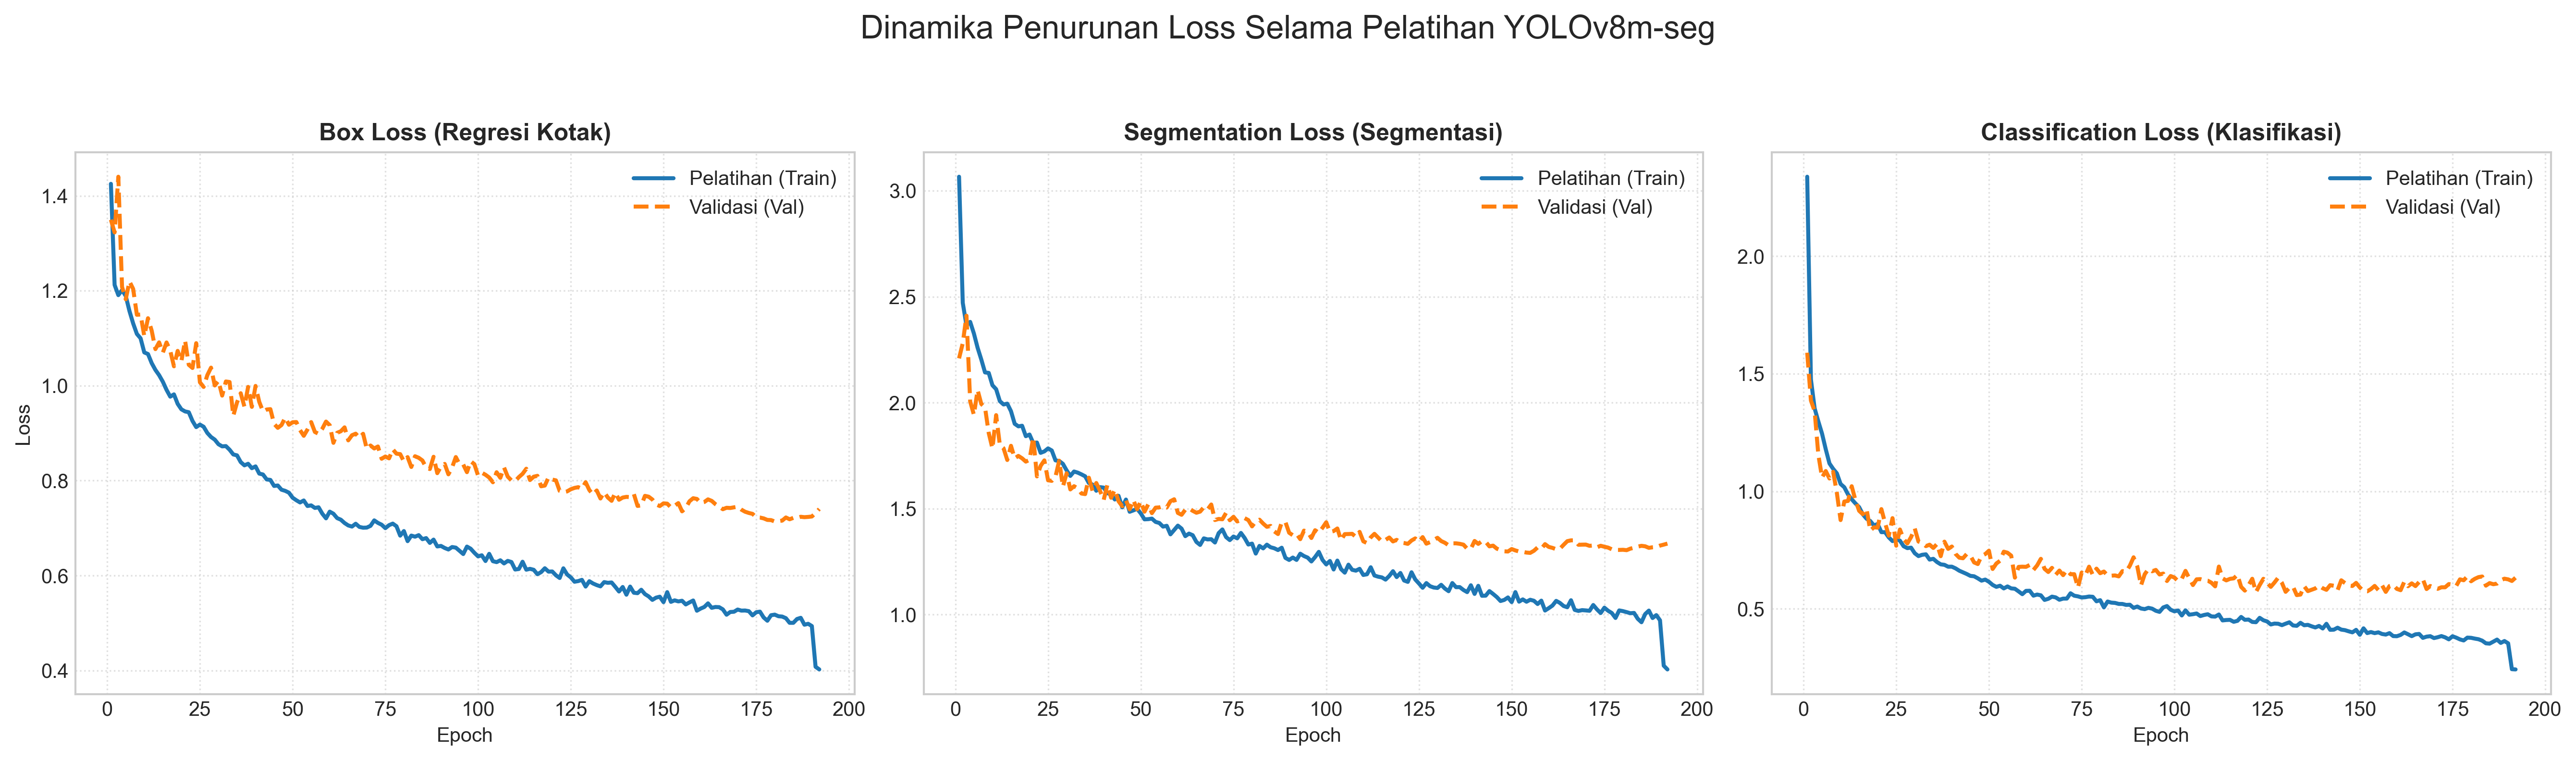
\includegraphics[width=\textwidth]{images/training_loss_custom.png} % Pastikan path sesuai
  \caption{Dinamika penurunan loss pelatihan dan validasi model YOLOv8m-seg. Grafik menunjukkan konvergensi yang stabil, di mana validasi loss (garis putus-putus oranye) mulai mendatar di sekitar epoch ke-92, memicu mekanisme early stopping setelah periode patience.}
  \label{fig:training_loss}
\end{figure}

\subsubsection{Evaluasi Metrik Kuantitatif dan Kualitatif}
\mbox{}\\
Evaluasi dilakukan pada dataset validasi berisi 300 citra dengan total 565 instansi objek. Tabel~\ref{tab:yolo_metrics} merangkum kinerja model berdasarkan metrik standar COCO. Secara agregat, model mencapai \textit{Mean Average Precision} (mAP) pada ambang batas IoU 0,5 sebesar \textbf{0,789}, yang menunjukkan ketahanan model yang tinggi.

\begin{table}[h]
\caption{\label{tab:yolo_metrics}Metrik Evaluasi Segmentasi YOLOv8m-seg pada Dataset Validasi.}
\begin{center}
\begin{tabular}{lcccc}
\toprule
Kelas & Precision (P) & Recall (R) & mAP@0.5 & mAP@0.5:0.95 \\
\midrule
\textbf{Semua Kelas} & \textbf{0.765} & \textbf{0.756} & \textbf{0.789} & \textbf{0.619} \\
Pothole & 0.795 & 0.912 & 0.892 & 0.685 \\
Manhole & 0.735 & 0.600 & 0.687 & 0.552 \\
\bottomrule
\end{tabular}
\end{center}
\end{table}

Analisis mendalam terhadap hasil tersebut mengungkapkan karakteristik performa berikut:
\begin{enumerate}
    \item \textbf{Prioritas Keselamatan (High Recall):} Skor \textit{Recall} sebesar \textbf{0,912} pada kelas \textit{Pothole} adalah indikator kinerja paling kritikal. Ini berarti sistem berhasil mendeteksi $>91\%$ anomali jalan, meminimalkan \textit{false negatives} yang berpotensi membahayakan pengguna jalan.
    \item \textbf{Kualitas Masker Segmentasi:} Nilai mAP@0.5:0.95 sebesar \textbf{0,619} (rata-rata di seluruh ambang IoU) mengonfirmasi bahwa masker segmentasi yang dihasilkan sangat ketat mengikuti kontur kerusakan yang ireguler. Presisi batas ini vital untuk akurasi perhitungan luas dan volume di tahap estimasi dimensi.
    \item \textbf{Analisis Matriks Kebingungan:} Berdasarkan analisis \textit{Confusion Matrix}, kesalahan klasifikasi antara \textit{Pothole} dan \textit{Manhole} sangat minim ($<2\%$). Kesalahan mayoritas berasal dari \textit{Background False Positives}, di mana bayangan pohon atau tambalan aspal terkadang terdeteksi sebagai lubang, namun hal ini dapat dimitigasi oleh filter CDKF pada tahap selanjutnya.
\end{enumerate}

Gambar~\ref{fig:detection_results} memvisualisasikan ketahanan model terhadap variasi pencahayaan dan oklusi parsial, membuktikan kelayakan model untuk penerapan di lingkungan nyata.

\begin{figure}[H]
  \centering
  
\includegraphics[width=\textwidth]{images/val_batch1_pred.jpg}
  \caption{Visualisasi hasil deteksi dan segmentasi pada data uji (validasi). Model berhasil memprediksi bounding box dan masker segmentasi untuk lubang jalan dengan akurasi tinggi.}
  \label{fig:detection_results}
\end{figure}




\subsection{Akurasi Pengukuran Dimensi}

\subsection{Performa Sistem Real-time}

\section{Kesimpulan}
\label{sec:conclusion}

\ack
Penulis ingin mengucapkan terima kasih kepada Departemen Sistem Informasi Universitas Hasanuddin atas dukungan dan sumber daya yang diberikan selama penelitian ini.


\begin{thebibliography}{00}

\bibitem{kemenpupr}
Kementerian Pekerjaan Umum dan Perumahan Rakyat (PUPR), ``Statistik Jalan Indonesia,'' 2024. [Daring]. Tersedia: https://pu.go.id

\bibitem{aharon2022}
N. Aharon, A. Bewley, and L. Zhang, ``BoT-SORT: Robust associations multi-pedestrian tracking,'' \emph{arXiv preprint arXiv:2206.14651}, 2022. [Online]. Available: https://arxiv.org/abs/2206.14651

\bibitem{bentzer2025}
C. Bentzer, ``Evaluating Monocular Depth Estimation Methods for High-Resolution Road Infrastructure Inspection,'' KTH Royal Institute of Technology, 2025. [Online]. Available: https://kth.diva-portal.org/smash/get/diva2:1987417/FULLTEXT01.pdf

\bibitem{depthanything2024}
L. Yang, B. Kang, Z. Huang, X. Xu, J. Feng, and H. Zhao, ``Depth Anything V2,'' \emph{arXiv preprint arXiv:2406.09414}, 2024. [Online]. Available: https://arxiv.org/abs/2406.09414

\bibitem{florea2025}
H. Florea and S. Nedevschi, ``TanDepth: Leveraging Global DEMs for Metric Monocular Depth Estimation in UAVs,'' \emph{IEEE J. Sel. Top. Appl. Earth Obs. Remote Sens.}, 2025. [Online]. Available: https://arxiv.org/abs/2409.05142

\bibitem{gorro2024}
J. Gorro, X. Li, and A. Rahman, ``JOIG: YOLOv8 + Augmentation for Pothole Detection,'' \emph{Journal of Object and Image Geometry}, vol. 12, no. 3, pp. 45--57, 2024.

\bibitem{hoseini2024}
M. Hoseini, P. Zhang, and R. Farahani, ``Deep learning architectures for real-time object detection,'' \emph{International Journal of Computer Vision and Applications}, vol. 8, no. 2, pp. 101--113, 2024.

\bibitem{laina2016}
I. Laina, C. Rupprecht, V. Belagiannis, F. Tombari, and N. Navab, ``Deeper depth prediction with fully convolutional residual networks,'' in \emph{Proc. IEEE Int. Conf. 3D Vision (3DV)}, 2016, pp. 239--248.

\bibitem{ranftl2021}
R. Ranftl, K. Lasinger, D. Hafner, K. Schindler, and V. Koltun, ``Vision transformers for dense prediction,'' in \emph{Proc. IEEE/CVF Int. Conf. Comput. Vision (ICCV)}, 2021, pp. 12179--12188.

\bibitem{wang2025}
D. Wang, H. Zhu, Y. Xu, and K. Liu, ``Integrated monocular depth estimation with temporal filtering for robust measurement,'' \emph{arXiv preprint arXiv:2505.21049}, 2025. [Online]. Available: https://arxiv.org/abs/2505.21049

\bibitem{singh2021}
R. Singh and N. Gupta, ``Pothole Detection and Dimension Estimation System using Deep Learning YOLO and Image Processing,'' \emph{Int. J. Comput. Appl.}, vol. 174, no. 12, pp. 12--18, 2021.

\bibitem{zhang2020}
T. Zhang and L. Chen, ``Rethinking Road Surface 3D Reconstruction and Pothole Detection,'' \emph{arXiv preprint arXiv:2012.10802}, 2020. [Online]. Available: https://arxiv.org/abs/2012.10802

\bibitem{rahman2025}
F. Rahman and U. Javed, ``An Analysis of Kalman Filter-based Object Tracking Methods for Fast-Moving Tiny Objects,'' \emph{ResearchGate Preprint}, 2025. [Online]. Available: https://www.researchgate.net/publication/395771559

\end{thebibliography}

\end{document}
